%% ANNP Algorithm Overview and Principles
%% XeLaTeX preprint draft — single section
%% Compile with: xelatex annp_algorithm.tex

\documentclass[11pt,a4paper]{article}

\usepackage{fontspec}
\setmainfont{LibertinusSerif-Regular.otf}[
  Path            = /usr/share/fonts/libertinus-fonts/,
  BoldFont        = LibertinusSerif-Bold.otf,
  ItalicFont      = LibertinusSerif-Italic.otf,
  BoldItalicFont  = LibertinusSerif-BoldItalic.otf
]
\setmonofont{LibertinusMono-Regular.otf}[
  Path  = /usr/share/fonts/libertinus-fonts/,
  Scale = 0.85
]

\usepackage{amsmath,amssymb,amsthm}
\usepackage{mathtools}
\usepackage{geometry}
\geometry{margin=2.5cm}
\usepackage{microtype}
\usepackage{hyperref}
\hypersetup{colorlinks=true, linkcolor=blue!70!black, urlcolor=blue!70!black, citecolor=red!60!black}
\usepackage{graphicx}
\usepackage{xcolor}
\usepackage{booktabs}
\usepackage{array}
\usepackage{multirow}
\usepackage{algorithm}
\usepackage{algpseudocode}
\usepackage{tikz}
\usetikzlibrary{arrows.meta, positioning, shapes.geometric, decorations.pathreplacing, calc, fit, backgrounds}
\usepackage{pgfplots}
\pgfplotsset{compat=1.18}
\usepackage{tcolorbox}
\tcbuselibrary{skins, breakable}
\usepackage{enumitem}
\usepackage{subcaption}

%% Custom theorem environments
\theoremstyle{definition}
\newtheorem{definition}{Definition}[section]
\newtheorem{proposition}{Proposition}[section]
\newtheorem{remark}{Remark}[section]

%% Design callout box
\newtcolorbox{designbox}[2][]{
  colback=blue!4!white,
  colframe=blue!40!black,
  fonttitle=\bfseries\small,
  title={#2},
  #1
}

\newtcolorbox{mathbox}[2][]{
  colback=gray!5!white,
  colframe=gray!50!black,
  fonttitle=\bfseries\small,
  title={#2},
  #1
}

%% Notation macros
\newcommand{\vp}{\mathbf{p}}
\newcommand{\vq}{\mathbf{q}}
\newcommand{\vx}{\mathbf{x}}
\newcommand{\vy}{\mathbf{y}}
\newcommand{\vs}{\mathbf{s}}
\newcommand{\va}{\mathbf{a}}
\newcommand{\vd}{\mathbf{d}}
\newcommand{\mW}{\mathbf{W}}
\newcommand{\mG}{\mathbf{G}}
\newcommand{\mU}{\mathbf{U}}
\newcommand{\mD}{\mathbf{D}}
\newcommand{\R}{\mathbb{R}}
\newcommand{\E}{\mathbb{E}}
\newcommand{\norm}[1]{\left\lVert #1 \right\rVert}
\newcommand{\RMSNorm}{\mathrm{RMSNorm}}
\newcommand{\swish}{\mathrm{swish}}
\newcommand{\clamp}{\mathrm{clamp}}
\DeclareMathOperator*{\argmax}{argmax}

\title{\textbf{Asynchronous Decentralized Neural Network Particles (ANNP):}\\
Algorithm Overview and Principles}
\author{[Anonymised for Draft]}
\date{\today\ --- Internal Draft}

\begin{document}
\maketitle
\tableofcontents
\newpage

%% ============================================================
\section{Algorithm Overview and Principles}
\label{sec:algorithm}
%% ============================================================

\subsection{Motivation and Design Philosophy}
\label{sec:motivation}

Contemporary large language models rely on the Transformer architecture, whose core operations ---
multi-head self-attention with a global key-value cache, layer-norm, and dense feed-forward blocks ---
are fundamentally synchronous and centralized.
Every layer requires a globally consistent view of the full sequence, every head attends to the same
$(K,V)$ buffer, and learning updates are computed by a single monolithic backward pass propagated
through the entire computational graph.

ANNP departs from this paradigm along four structural axes:

\begin{enumerate}[leftmargin=2em]
  \item \textbf{Full decentralization.}
    There is no global hidden state, no shared key-value cache, and no centralized projection layer.
    Each compute cell makes decisions using only locally observable signals.
  \item \textbf{Emergent causality.}
    Causal structure is not hard-coded by an attention mask.
    It emerges from the temporal ordering implicit in the particle energy decay dynamics and
    the temporal-difference learning signal that only fires between causally ordered token pairs.
  \item \textbf{Hyperparameter minimalism.}
    Every free parameter in ANNP is either derived from the data distribution or computed from
    first principles. No learning-rate schedules, no warmup steps, no fixed-window decay constants,
    no hand-tuned softmax temperatures.
  \item \textbf{Continual learnability.}
    The architecture is designed to support online, incremental learning without catastrophic
    forgetting, achieved through structural rather than regularization-based mechanisms.
\end{enumerate}

\begin{designbox}{Design Invariant: KISS with Mathematical Grounding}
  When a design choice requires a free parameter, ANNP derives it from available statistics
  (e.g., $d_{\text{head}}$, cumulative energy $E_\text{cum}$) rather than setting it empirically.
  Empirical constants introduced only for implementation convenience are promoted to explicit
  configuration parameters with principled defaults, never silently hard-coded.
\end{designbox}

%% ============================================================
\subsection{System Architecture}
\label{sec:architecture}
%% ============================================================

\begin{figure}[ht]
\centering
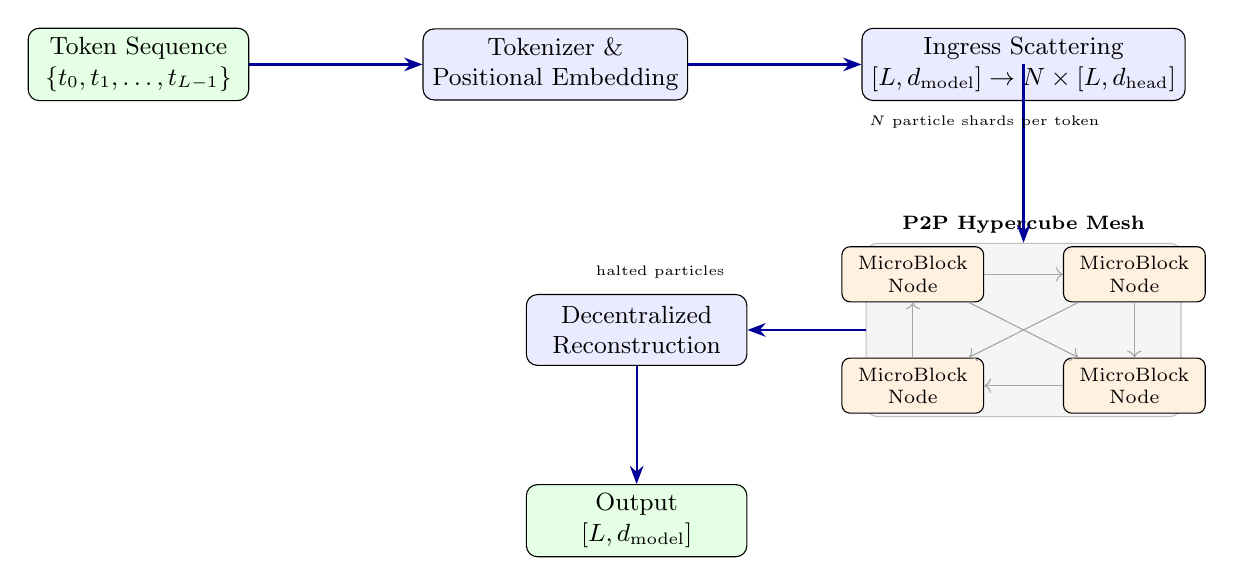
\begin{tikzpicture}[
  node distance=1.5cm and 2.2cm,
  block/.style={draw, rounded corners=4pt, fill=blue!8, minimum width=2.8cm, minimum height=0.9cm,
                align=center, font=\small},
  arrow/.style={-Stealth, thick, blue!60!black},
  smallblock/.style={draw, fill=orange!12, rounded corners=3pt, minimum width=1.8cm,
                     minimum height=0.7cm, align=center, font=\scriptsize}
]
  %% Input
  \node[block, fill=green!10] (input) {Token Sequence\\$\{t_0, t_1, \ldots, t_{L-1}\}$};

  %% Tokenizer
  \node[block, right=of input] (tok) {Tokenizer \&\\Positional Embedding};

  %% Scattering
  \node[block, right=of tok] (scatter) {Ingress Scattering\\$[L, d_\text{model}] \to N \times [L, d_\text{head}]$};

  %% Mesh
  \node[block, below=1.8cm of scatter, minimum width=4cm, minimum height=2.2cm, fill=gray!8,
        draw=gray!50] (mesh) {};
  \node[above=0pt of mesh.north, font=\scriptsize\bfseries] {P2P Hypercube Mesh};

  \node[smallblock, at=(mesh.north west), xshift=0.6cm, yshift=-0.4cm] (n1) {MicroBlock\\Node};
  \node[smallblock, at=(mesh.north east), xshift=-0.6cm, yshift=-0.4cm] (n2) {MicroBlock\\Node};
  \node[smallblock, at=(mesh.south west), xshift=0.6cm, yshift=0.4cm] (n3) {MicroBlock\\Node};
  \node[smallblock, at=(mesh.south east), xshift=-0.6cm, yshift=0.4cm] (n4) {MicroBlock\\Node};

  \draw[->, gray!70, thin] (n1) -- (n2); \draw[->, gray!70, thin] (n2) -- (n4);
  \draw[->, gray!70, thin] (n4) -- (n3); \draw[->, gray!70, thin] (n3) -- (n1);
  \draw[->, gray!70, thin] (n1) -- (n4); \draw[->, gray!70, thin] (n2) -- (n3);

  %% Reconstruction
  \node[block, left=1.5cm of mesh] (recon) {Decentralized\\Reconstruction};

  %% Output
  \node[block, below=of recon, fill=green!10] (output) {Output\\$[L, d_\text{model}]$};

  %% Arrows
  \draw[arrow] (input) -- (tok);
  \draw[arrow] (tok) -- (scatter);
  \draw[arrow] (scatter) -- (scatter -| mesh.north) -- (mesh.north);
  \draw[arrow] (mesh.west) -- (recon);
  \draw[arrow] (recon) -- (output);

  %% Labels
  \node[font=\tiny, below=2pt of scatter, xshift=-0.5cm] {$N$ particle shards per token};
  \node[font=\tiny, above=2pt of recon, xshift=0.3cm] {halted particles};
\end{tikzpicture}
\caption{%
  End-to-end ANNP pipeline.
  A token sequence is embedded with positional encoding, then split into $N$ parallel particle shards
  which propagate through a structured P2P mesh of decentralized compute cells.
  Particles that halt (by energy exhaustion or spontaneous settling) are gathered and reassembled
  into the output representation without any centralized projection.
}
\label{fig:pipeline}
\end{figure}

ANNP organizes computation into four layers:

\begin{enumerate}[leftmargin=2em]
  \item \textbf{Tokenization and positional embedding.} (\S\ref{sec:tokenizer})
  \item \textbf{Ingress scattering.} Token embeddings are split into $N$ independent particle shards
    and injected into the mesh at uniformly distributed ingress nodes. (\S\ref{sec:scattering})
  \item \textbf{Decentralized P2P mesh routing and computation.}
    Particles propagate through the mesh, processed at each visited node by the MicroBlock operator.
    (\S\ref{sec:mesh}--\S\ref{sec:microblock})
  \item \textbf{Decentralized reconstruction.}
    Halted particles are assembled back into the output tensor with no learned projection. (\S\ref{sec:recon})
\end{enumerate}

%% ============================================================
\subsection{Tokenization and Positional Embedding}
\label{sec:tokenizer}
%% ============================================================

ANNP employs a deterministic, parameter-free token embedding.
For token $\tau$ at sequence position $\ell$ and model dimension $d_\text{model} = N \cdot d_\text{head}$,
the embedding is computed as follows.

First, a pseudo-random vector $\tilde{\vp}_\tau \in \R^{d_\text{model}}$ is generated using a
multiplicative Xorshift hash seeded by $\tau$:
\begin{equation}
  \text{seed}^{(0)} = \tau \cdot \texttt{0x9E3779B97F4A7C15} + 1,
  \qquad
  \tilde{p}_d = \text{Xorshift}(\text{seed}^{(d)}) \in [-1, 1].
  \label{eq:hash}
\end{equation}
The vector is then RMS-normalized to unit scale:
\begin{equation}
  \hat{\vp}_\tau = \frac{\tilde{\vp}_\tau}{\sqrt{\frac{1}{d}\sum_{d'} \tilde{p}_{d'}^2 + \varepsilon}}.
  \label{eq:toknorm}
\end{equation}
A sinusoidal positional signal is additively injected per dimension $d'$:
\begin{equation}
  e_{\tau,\ell,d'} = \hat{p}_{d'} + \sin\!\bigl(\ell \cdot f_0 + d' \cdot f_1\bigr) \cdot s_\text{enc},
  \label{eq:posenc}
\end{equation}
where $f_0 = 0.05$ (base token frequency), $f_1 = 0.01$ (dimension phase shift), and
$s_\text{enc} = 0.1$ are configurable.

\begin{remark}[Why parameter-free embeddings?]
  Learned embedding tables introduce an extra $|\mathcal{V}| \cdot d_\text{model}$ parameter block
  with its own initialization and optimization dynamics.
  The hash-based embedding is fully deterministic, avoids cold-start instability, and enables
  zero-shot generalization to unseen token IDs.
  The RMS normalization in \eqref{eq:toknorm} ensures $\norm{\hat{\vp}}_\text{RMS} \approx 1$
  regardless of $d_\text{model}$, preventing dimension-dependent energy imbalance.
\end{remark}

%% ============================================================
\subsection{Ingress Scattering}
\label{sec:scattering}
%% ============================================================

Given the embedding matrix $E \in \R^{L \times d_\text{model}}$ for a sequence of length $L$,
and $N$ nodes with $d_\text{head} = d_\text{model}/N$, the scattering operator decomposes
$E$ into $L \cdot N$ particle shards:
\begin{equation}
  \vp_{\ell,n} = E[\ell,\ n \cdot d_\text{head}\,:\, (n{+}1) \cdot d_\text{head}] \in \R^{d_\text{head}},
  \qquad \ell \in [L],\ n \in [N].
  \label{eq:scatter}
\end{equation}

Each particle $\vp_{\ell,n}$ carries a \emph{header} tuple
$(\text{origin\_token\_id},\ \text{shard\_id},\ E_\text{init},\ \text{hop})$ initialized to
$(\ell + \text{offset},\ n,\ E_\text{init},\ 0)$, where \texttt{offset} is the global cumulative
token count ensuring monotonically increasing token IDs across training sequences.

Particles are injected at a uniformly strided subset of $\lceil \rho \cdot N_\text{nodes} \rceil$
ingress nodes (controlled by ratio $\rho = \texttt{ingress\_ratio}$), with step size
$\lfloor N / n_\text{ingress} \rfloor$, to avoid clustering particles in a single topological region.

%% ============================================================
\subsection{Mesh Topology and Routing}
\label{sec:mesh}
%% ============================================================

\subsubsection{Structured Hypercube Connectivity}

The $N_\text{nodes}$ compute cells are connected by a structured mesh with topology diameter
$O(\sqrt{N_\text{nodes}})$, achieved by connecting node $i$ to
\begin{equation}
  \text{neighbors}(i) = \bigl\{(i + k \cdot s)\!\!\!\mod N_\text{nodes}
    : k = 1, 2, \ldots\bigr\},
  \qquad s = \lceil\sqrt{N_\text{nodes}}\rceil,
  \label{eq:topology}
\end{equation}
selecting $K$ distinct neighbors ($K = \texttt{k\_neighbors}$).
This generalizes a 2D-grid connectivity ($\sqrt{N}$-diameter) to arbitrary $N$,
in contrast to a ring topology whose diameter is $O(N)$.

\subsubsection{Decentralized Q-Routing with Thompson Sampling}

Each node maintains a local routing table $(\text{weights}, \text{edge\_credit})$.
The routing decision for an arriving particle $\vp$ at node $i$ selects neighbor $k^*$:
\begin{equation}
  k^* = \argmax_{k \in \mathcal{N}(i)}
  \underbrace{\vp^\top \mW_k}_{\text{content affinity}}
  +\, \underbrace{\mu_k + \sigma_k \cdot t_k}_{\text{Thompson sample}},
  \label{eq:routing}
\end{equation}
where $\mW_k \in \R^{d_\text{head}}$ is the content projection vector for neighbor $k$,
$\mu_k$ and $\sigma_k$ are the empirical posterior mean and standard error of $\Delta R$ credit
observations along edge $k$, and $t_k$ is sampled from a Student-$t$ approximation with $\nu_k = \max(1, n_k - 1)$ degrees of freedom.

When edge $k$ yields positive credit $\Delta R > 0$ for a transformed particle payload $\vp_\text{out}$,
the projection vector $\mW_k$ undergoes a Hebbian weight update:
\begin{equation}
  \mW_k \leftarrow \clamp\!\left(\mW_k + \eta_r \cdot \Delta R \cdot \hat{\vp}_\text{out},\, -w_\text{max},\, w_\text{max}\right),
  \qquad \eta_r = \frac{0.01}{d_\text{head}},
  \label{eq:routing_hebbian}
\end{equation}
where $\hat{\vp}_\text{out} = \RMSNorm(\vp_\text{out})$ and $w_\text{max} = 3/\sqrt{d_\text{head}}$.
This enables $\mW_k$ to dynamically align with the semantic manifold of particles that receive positive credit at neighbor $k$, preventing high-credit nodes from degenerating into semantic-blind traffic hubs.

\begin{designbox}{Content + Credit: Two-Signal Routing}
  Pure content routing ($\vp^\top \mW_k$ alone) ignores whether neighbor $k$ is
  currently processing useful transformations.
  Pure credit routing ignores particle-node semantic compatibility.
  The combined signal \eqref{eq:routing} routes particles both to contextually matching nodes
  and to nodes with proven recent performance, without requiring any additional hyperparameter.
\end{designbox}

\paragraph{Posterior approximation.}
Credit statistics are maintained using an exponential-decay Welford algorithm.
Given EMA decay $\gamma = 1 - 1/d_\text{head}^2$, the effective observation window is
$N_\text{eff} = 1/(1-\gamma) = d_\text{head}^2$,
aligning the routing credit memory with the size of the local fast-weight associative memory.

\paragraph{Exploration decay.}
New edges and freshly spawned subnodes receive an infinite prior score on the first selection,
guaranteeing at least one evaluation before competing on observed merits (multi-armed bandit
optimistic initialization).
As $n_k$ grows, the Student-$t$ distribution's heavy tails contract toward Gaussian,
automatically shifting from exploration to exploitation without any explicit schedule.

\paragraph{Link pruning.}
Routing links are pruned using $2\sigma$ confidence intervals: link $k$ is removed when
its upper confidence bound $\mu_k + 2\sigma_k$ falls below the best link's lower confidence
bound $\max_j(\mu_j - 2\sigma_j)$, requiring statistical significance rather than raw mean comparison.

\paragraph{Backpressure.}
If the target queue exceeds $B_\text{max} = \texttt{queue\_backpressure}$ particles,
the particle overflows to a neighbor from the local adjacency list, selected by
$(\text{hop\_count} \mod |\mathcal{N}|)$ to distribute load without centralized coordination.

%% ============================================================
\subsection{Particle Energy Dynamics}
\label{sec:energy}
%% ============================================================

Each particle carries energy $E(h) \in [0, E_\text{init}]$ decaying linearly with hop count $h$:
\begin{equation}
  E(h) = E_\text{init} - h \cdot \frac{E_\text{init}}{h_\text{max}} = E_\text{init}\!\left(1 - \frac{h}{h_\text{max}}\right).
  \label{eq:energy}
\end{equation}
The particle halts (is collected) when $E(h) \le 0$ or $h \ge h_\text{max}$.

\begin{remark}[Linear vs.\ exponential decay]
  Exponential decay $E(h) = E_0 \cdot \rho^h$ requires a threshold $\varepsilon$ to determine
  when the particle is ``close enough to zero'', introducing a hidden hyperparameter.
  Linear decay \eqref{eq:energy} guarantees $E(h_\text{max}) = 0$ exactly: the particle lifetime
  equals $h_\text{max}$ without any implicit threshold.
  A single interpretable parameter $h_\text{max}$ controls the average propagation depth.
\end{remark}

\paragraph{Spontaneous halting.}
Independently of energy exhaustion, a particle halts spontaneously if it receives negative
credit ($\Delta R < 0$) for $k_\text{halt}$ consecutive sub-batches at the current node:
\begin{equation}
  \text{halt if} \quad \Delta R_{h-k_\text{halt}+1} \le 0 \;\wedge\; \cdots \;\wedge\; \Delta R_h \le 0,
  \quad k_\text{halt} = \texttt{early\_halt\_streak}.
  \label{eq:spontaneous}
\end{equation}
This implements a local convergence criterion: $k_\text{halt}$ consecutive negative credits
provides stronger evidence of settled state than a single observation, reducing sensitivity to
transient noise. The default $k_\text{halt} = 2$ is the minimal streak that filters single-sample
noise while remaining responsive.

%% ============================================================
\subsection{The MicroBlock Node}
\label{sec:microblock}
%% ============================================================

The \emph{MicroBlock Node} is the fundamental compute cell.
Each node independently maintains three learnable structures: (i) a fast-weight associative memory
$\mW_\text{fw} \in \R^{d_\text{head} \times d_\text{head}}$, (ii) a pool of competing FFN
specializations called \emph{subnodes}, and (iii) temporal-difference state.

\subsubsection{Forward Computation}

On receiving a sub-batch of particles sharing the same origin token $\ell$,
the node aggregates their payloads into a mean input:
\begin{equation}
  \bar{\vp}_\text{in} = \frac{1}{|B|}\sum_{i \in B} \vp_i.
  \label{eq:aggregate}
\end{equation}
The aggregated input is RMS-normalized:
\begin{equation}
  \hat{\vp}_\text{in} = \RMSNorm(\bar{\vp}_\text{in})
    = \frac{\bar{\vp}_\text{in}}{\sqrt{\frac{1}{d}\norm{\bar{\vp}_\text{in}}^2 + \varepsilon}}.
  \label{eq:rmsnorm}
\end{equation}
The fast-weight attention produces a context vector:
\begin{equation}
  \va_\text{out} = \mW_\text{fw} \, \hat{\vp}_\text{in} \in \R^{d_\text{head}}.
  \label{eq:fwa}
\end{equation}
The active subnode (selected by Thompson Sampling; see \S\ref{sec:subnodes}) applies a
SwiGLU-style gated FFN to the residual-attended state:
\begin{equation}
  \vs_\text{mid} = \bar{\vp}_\text{in} + \alpha \cdot \va_\text{out},
  \label{eq:smid}
\end{equation}
\begin{equation}
  \text{FFN}(\vs) = \mD\,\bigl[\swish(\mG\,\RMSNorm(\vs)) \odot (\mU\,\RMSNorm(\vs))\bigr],
  \qquad \swish(x) = x \cdot \sigma(x),
  \label{eq:ffn}
\end{equation}
\begin{equation}
  \vp_\text{out} = \vs_\text{mid} + \alpha \cdot \text{FFN}(\vs_\text{mid}),
  \label{eq:pout}
\end{equation}
where $\mG, \mU \in \R^{d_\text{head} \times d_\text{ffn}}$,
$\mD \in \R^{d_\text{ffn} \times d_\text{head}}$, $d_\text{ffn} = d_\text{head} \cdot f_\text{expand}$,
and $\alpha$ is the subnode's residual scale.

\paragraph{Energy conservation.}
Without normalization, the residual update
$\vp_\text{out} = \vp_\text{in} + \alpha \cdot \text{FFN}(\vp_\text{in})$ inflates the
signal energy by a factor of $\approx(1+\alpha^2)$ per hop.
After $K$ hops this produces exponential amplification.
The particle payload is re-scaled by
\begin{equation}
  \vp_\text{payload} \leftarrow \frac{\vp_\text{out}}{\sqrt{1 + \alpha^2}},
  \label{eq:scale}
\end{equation}
which keeps expected energy approximately constant:
$\E[\norm{\vp_\text{payload}}^2] \approx \E[\norm{\vp_\text{in}}^2]$.
This is the KISS principle applied to energy stability: no separate LayerNorm on the propagating
signal.

\subsubsection{Fast-Weight Associative Memory and Hardening}
\label{sec:fastweight}

The fast-weight matrix $\mW_\text{fw}$ is a local Hopfield-style associative memory.
It is initialized to small random values at Kaiming scale $1/d_\text{head}$
(not zeros, to avoid the cold-start credit deadlock described in \S\ref{sec:credit}).

The update rule is Hebbian with energy-driven retention hardening:
\begin{equation}
  \mW_\text{fw} \leftarrow \lambda \cdot \mW_\text{fw} - \eta \cdot \clamp\!\left(g, -g_\text{max}, g_\text{max}\right),
  \label{eq:fwupdate}
\end{equation}
\begin{equation}
  \lambda = 1 - \frac{1}{\sqrt{E_\text{cum}}},
  \label{eq:lambda}
\end{equation}
where $E_\text{cum} = \sum_t \norm{\vp_\text{in}^{(t)}}^2$ is the cumulative squared input energy
and $g$ is the gradient computed via the TD chain (see \S\ref{sec:td}).

\begin{designbox}{Why $\lambda = 1 - 1/\sqrt{E_\text{cum}}$ is not a hyperparameter}
  The retention factor $\lambda$ is derived from the node's empirical signal experience:
  \begin{itemize}[itemsep=0pt]
    \item \textbf{Early phase} ($E_\text{cum}$ small): $\lambda \approx 0$, fast-weight decays aggressively.
      The node is still plastic; it should not over-retain early noisy observations.
    \item \textbf{Mature phase} ($E_\text{cum}$ large): $\lambda \to 1$, fast-weight retains associations.
      The node has accumulated significant, high-quality signal and should stabilize.
    \item \textbf{Data-quality sensitivity}: $E_\text{cum}$ reflects signal energy (amplitude),
      not token count. Nodes receiving strong structured inputs harden faster than nodes
      receiving diffuse low-energy particles --- a desirable property absent from token-count-based schedules.
  \end{itemize}
\end{designbox}

\subsubsection{Local Credit Signal: $\Delta R$ Resonance}
\label{sec:credit}

The sole routing-learning signal is the change in fast-weight resonance induced by the node's
transformation.
For particle $\vp$ before and after processing:
\begin{equation}
  \Delta R = R_\text{after} - R_\text{before},
  \qquad
  R(\vp) = \hat{\vp}^\top \mW_\text{fw}\, \hat{\vp},
  \qquad \hat{\vp} = \RMSNorm(\vp).
  \label{eq:credit}
\end{equation}

$\Delta R > 0$ means the transformation moved the particle payload toward directions reinforced
in the fast-weight memory: the node's computation was beneficial for this particle.
$\Delta R < 0$ indicates the particle was pushed away from familiar patterns.

\begin{mathbox}{Cold-Start Prevention}
  If $\mW_\text{fw} = \mathbf{0}$ at initialization, then $R(\vp) = 0$ for any $\vp$,
  so $\Delta R \equiv 0$ before any Hebbian updates accumulate.
  With no credit signal, routing is uninformative and learning stalls.
  Initializing $\mW_\text{fw}$ with values from $\mathcal{U}(-1/d_\text{head}, 1/d_\text{head})$
  produces an initial quadratic form magnitude $|R| \sim O(1/d_\text{head})$,
  small enough not to distort early computation but sufficient to break the deadlock.
\end{mathbox}

\subsubsection{Temporal-Difference Learning}
\label{sec:td}

Each subnode $j$ independently maintains its own temporal-difference state
$\bigl(\bar{\vp}_\text{last}^{(j)},\, \hat{\vp}_\text{pred}^{(j)},\, \ell_\text{last}^{(j)}\bigr)$.
When subnode $j$ is active for a sub-batch at token $\ell > \ell_\text{last}^{(j)}$, the TD error is computed against subnode $j$'s own previous activation:
\begin{equation}
  \boldsymbol{\delta}^{(j)} = w(dt) \cdot \bigl(\hat{\vp}_\text{pred}^{(j)} - \bar{\vp}_\text{in}^\ell\bigr),
  \qquad w(dt) = \frac{1}{dt},\quad dt = \ell - \ell_\text{last}^{(j)}.
  \label{eq:tderror}
\end{equation}
By isolating TD prediction states to individual specialized subnodes, temporal-difference signals remain uncorrupted by heterogeneous particle streams visiting the same container node.
The local loss at step $\ell$ is the mean-squared TD error:
\begin{equation}
  \mathcal{L}_\ell = \frac{1}{d_\text{head}} \norm{\boldsymbol{\delta}}^2.
  \label{eq:loss}
\end{equation}

Backpropagation through \eqref{eq:pout}--\eqref{eq:rmsnorm} computes gradients
$\partial \mathcal{L}_\ell / \partial \mD,\, \partial \mathcal{L}_\ell / \partial \mG,\,
\partial \mathcal{L}_\ell / \partial \mU,\, \partial \mathcal{L}_\ell / \partial \mW_\text{fw}$,
applied with L2 weight decay:
\begin{equation}
  \theta \leftarrow (1 - \eta \cdot \lambda_\text{wd}) \cdot \theta - \eta \cdot \nabla_\theta \mathcal{L}.
  \label{eq:update}
\end{equation}

\begin{remark}[Harmonic discount $1/dt$ avoids hyperparameters]
  Standard temporal-difference methods use exponential discount $\gamma^{dt}$,
  requiring choice of $\gamma$.
  The harmonic weight $w(dt) = 1/dt$ requires no such choice:
  adjacent tokens ($dt=1$) receive full weight, distant tokens vanish naturally without
  explicit truncation. This is analogous to the $1/r$ potential in one dimension.
  The guard $\ell > \ell_\text{last}$ ensures only forward (causal) predictions are learned,
  and the use of globally monotone token IDs prevents cross-sequence confounding.
\end{remark}

\begin{remark}[No frequency-based learning rate decay]
  A naive adaptation of AdaGrad/Adam with $\eta_j = \eta / \sqrt{S_j}$ (where $S_j$ counts
  activations at node $j$) fails in ANNP because $S_j$ grows by $|B| \cdot h_\text{avg}$ per
  forward call ($\approx 100\text{--}500$ per call). After a single forward pass,
  $\eta_j$ is already reduced to near zero, effectively freezing the weights.
  Instead, ANNP relies on three structural mechanisms for stability and anti-forgetting:
  (1) routing dynamics naturally reinforce high-credit nodes;
  (2) the data-quality-adaptive $\lambda(E_\text{cum})$ hardens only well-stimulated associations;
  (3) L2 weight decay \eqref{eq:update} prevents unbounded weight growth.
\end{remark}

\subsubsection{Gradient Clipping}
All gradient components are clamped element-wise to $[-g_\text{max}, g_\text{max}]$ with
\begin{equation}
  g_\text{max} = \frac{1}{\sqrt{d_\text{head}}},
  \label{eq:gradclip}
\end{equation}
which is the natural scale of the product of two unit-scale vectors (one gradient, one activation).
This prevents gradient spikes without requiring a global gradient norm, consistent with decentralization.

%% ============================================================
\subsection{Subnode Competition and Cellular Neurogenesis}
\label{sec:subnodes}
%% ============================================================

Each MicroBlock node hosts between 1 and $K_\text{max}$ \emph{subnodes}, each a distinct
SwiGLU FFN specialization. Subnodes compete for activation via Thompson Sampling and undergo
biological-style neurogenesis and pruning.

\subsubsection{Subnode Initialization}

A subnode's FFN weights are initialized by He/Kaiming scaling:
\begin{equation}
  \mG, \mU \sim \mathcal{U}\!\left(-s, s\right),
  \quad s = \sqrt{\frac{2}{d_\text{head} + d_\text{ffn}}},
  \label{eq:init_gate}
\end{equation}
\begin{equation}
  \mD \sim \mathcal{U}\!\left(-s_D, s_D\right),
  \quad s_D = \frac{s}{\sqrt{d_\text{head}}}.
  \label{eq:init_down}
\end{equation}
The additional $1/\sqrt{d_\text{head}}$ factor on $\mD$ keeps
$\mathrm{Var}(\text{FFN output}) \approx 1$ at initialization,
preventing the FFN residual from dominating the input at small $\alpha$.
The residual scale is initialized to $\alpha_0 = 1/\sqrt{d_\text{head}}$.

\subsubsection{Thompson Sampling Selection}

At each sub-batch, the active subnode is selected by drawing from each subnode's empirical
credit posterior:
\begin{equation}
  \text{score}_j =
  \begin{cases}
    +\infty & \text{if } n_j \le 1 \quad\text{(guaranteed first evaluation)}, \\
    \mu_j + \mathrm{SE}_j \cdot t_j & \text{otherwise},
  \end{cases}
  \label{eq:thompson}
\end{equation}
\begin{equation}
  t_j \sim \mathrm{Student\text{-}t}(\nu_j),
  \quad \nu_j = \max(1,\, n_j - 1),
  \quad \mathrm{SE}_j = \sqrt{\mathrm{Var}_j / n_j}.
  \label{eq:tstat}
\end{equation}

\begin{designbox}{Student-$t$ over Gaussian Thompson Sampling}
  At small $\nu_j$ (early learning), the Student-$t$ distribution has heavy tails,
  enabling rare but informative explorations of uncertain subnodes.
  As $\nu_j$ grows, it converges to the normal distribution, automatically shifting to
  exploitation. No exploration coefficient $c$ is required, unlike UCB methods.
  The approximation uses a first-order Cornish-Fisher expansion, avoiding external dependencies.
\end{designbox}

\subsubsection{Health Dynamics}

Every subnode $j$ maintains a scalar viability \emph{health} $h_j \ge 0$.
At each sub-batch, all subnodes lose health by a fixed rate:
\begin{equation}
  h_j \leftarrow h_j - \frac{1}{d_\text{head}},
  \label{eq:decay}
\end{equation}
regardless of population size.
The selected subnode $j^*$ additionally recovers:
\begin{equation}
  h_{j^*} \leftarrow h_{j^*} + \frac{\alpha_{j^*}}{d_\text{head}} + \Delta h_\text{credit},
  \label{eq:recovery}
\end{equation}
\begin{equation}
  \Delta h_\text{credit} =
  \begin{cases}
    \bar{\Delta R} & \text{if } \bar{\Delta R} > 0, \\
    \lambda_{j^*} \cdot \beta_d \cdot \bar{\Delta R} & \text{if } \bar{\Delta R} \le 0,
  \end{cases}
  \label{eq:credhealth}
\end{equation}
where $\bar{\Delta R}$ is the mean batch credit, $\beta_d = \texttt{negative\_credit\_damping}$ is the damping factor, and $\lambda_{j^*} = 1 - 1/\sqrt{E_{\text{cum}}^{(j^*)}}$ is the subnode's memory maturity. Plastic newborn subnodes ($\lambda_{j^*} \approx 0$) receive zero death penalty on initial weight perturbations, allowing gradient updates to adapt their plastic weights towards positive resonance, while mature subnodes ($\lambda_{j^*} \to 1$) face full accountability.

\begin{remark}[Fixed decay rate vs.\ population-proportional]
  If the decay were $1/(d_\text{head} \cdot |\text{subnodes}|)$, adding more subnodes would
  slow each one's decay, letting weak subnodes survive longer purely by being numerous ---
  a positive feedback loop that undermines natural selection.
  The fixed rate $1/d_\text{head}$ ensures each subnode competes on intrinsic merit.
\end{remark}

\subsubsection{Neurogenesis and Pruning}

\paragraph{Neurogenesis.}
A split event occurs when three conditions are simultaneously satisfied:
\begin{enumerate}[itemsep=0pt]
  \item \textbf{Capacity:} $|\text{subnodes}| < K_\text{max}$.
  \item \textbf{Vitality:} $h_{j^*} > h_\text{base} \cdot (1 + |\text{subnodes}|)$.
  \item \textbf{Information variance:} $n_{j^*} > 1$ and $\mathrm{Var}_{j^*} > 0$.
\end{enumerate}
A child subnode is spawned with weights perturbed from the parent by
$\varepsilon = 1/\sqrt{d_\text{head} \cdot d_\text{ffn}}$:
\begin{equation}
  \theta_\text{child} = \theta_\text{parent} + \mathcal{U}(-\varepsilon, \varepsilon).
  \label{eq:perturb}
\end{equation}
The perturbation $\varepsilon \approx 10\%$ of the initial weight magnitude
$s \approx \sqrt{2/(d+d_\text{ffn})}$, providing sufficient diversity for divergent
specialization while preserving the parent's learned functional scale.
The parent's health is halved upon spawning ($h_{j^*} \leftarrow h_{j^*}/2$),
modeling the energetic cost of cell division.
The newborn is initialized with an embryonic health reserve:
\begin{equation}
  h_\text{child,init} = d_\text{head} \cdot h_\text{base},
  \label{eq:child_health_init}
\end{equation}
which is dimensionally paired with the passive decay rate $1/d_\text{head}$ per batch, giving a
runway of $d_\text{head}^2 \cdot h_\text{base}$ batches.
This interval is commensurate with filling the $d_\text{head} \times d_\text{head}$ associative
memory once \textemdash{} sufficient for gradient updates to differentiate the child's plastic
weights before it enters fair Thompson Sampling competition.
No new hyperparameters are introduced; $d_\text{head}$ and $h_\text{base}$ are pre-existing
structural parameters.

The child inherits $\alpha_\text{parent}$ (not re-randomized), since $\alpha$ encodes the
correct operating scale; re-discovery from scratch would delay specialization.
Crucially, the child inherits the parent's empirical credit statistics $(\mu_\text{parent},\, \text{Var}_\text{parent})$ with virtual count set to $n_\text{child} = 2.0$.
This yields degrees of freedom $\nu_\text{child} = n_\text{child} - 1 = 1$, where the Student-$t$ distribution reduces to a heavy-tailed Cauchy distribution.
Inheriting non-zero prior variance ensures $\mathrm{SE}_\text{child} = \sqrt{\mathrm{Var} / 2} > 0$, allowing Cauchy heavy tails to generate natural Bayesian exploration opportunities while the newborn's fully plastic weights ($E_{\text{cum}}^{(\text{child})} = 0 \implies \lambda_{\text{child}} = 0$) adapt to the new manifold. Zero extra hyperparameters are introduced.

\paragraph{Pruning.}
Subnodes with $h_j \le 0$ are eliminated after each full batch.
At least one subnode is always retained (the healthiest) to preserve node viability.
The pruning criterion is deterministic and requires no threshold hyperparameter.

\begin{figure}[ht]
\centering
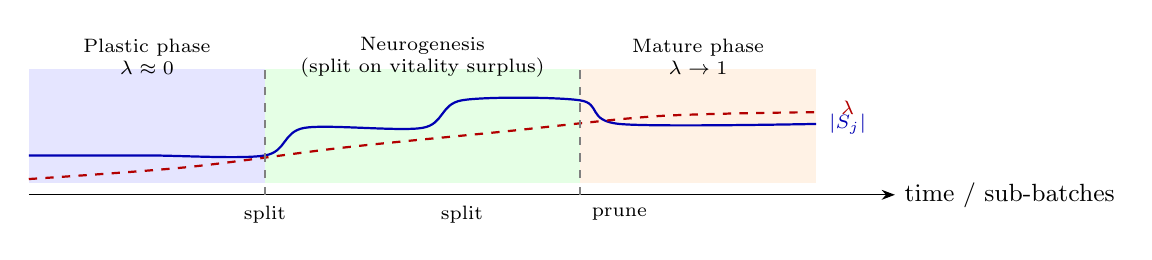
\begin{tikzpicture}[>=Stealth, font=\small]
  % Timeline axis
  \draw[->] (0,0) -- (11,0) node[right]{time / sub-batches};

  % Phases
  \fill[blue!10] (0,0.15) rectangle (3,1.6);
  \fill[green!10] (3,0.15) rectangle (7,1.6);
  \fill[orange!10] (7,0.15) rectangle (10,1.6);

  \node[font=\scriptsize, align=center] at (1.5, 1.75) {Plastic phase\\$\lambda \approx 0$};
  \node[font=\scriptsize, align=center] at (5, 1.75) {Neurogenesis\\(split on vitality surplus)};
  \node[font=\scriptsize, align=center] at (8.5, 1.75) {Mature phase\\$\lambda \to 1$};

  % Subnode count curve
  \draw[blue!70!black, thick] plot[smooth] coordinates
    {(0,0.5) (1.5,0.5) (3,0.5) (3.5,0.85) (5,0.85) (5.5,1.2) (7,1.2) (7.5,0.9) (10,0.9)};
  \node[blue!70!black, font=\scriptsize] at (10.4, 0.9) {$|S_j|$};

  % Lambda curve
  \draw[red!70!black, dashed, thick] plot[smooth] coordinates
    {(0,0.2) (2,0.35) (4,0.6) (6,0.8) (8,1.0) (10,1.05)};
  \node[red!70!black, font=\scriptsize] at (10.4, 1.1) {$\lambda$};

  % Annotations
  \draw[dashed, gray] (3,0) -- (3,1.6);
  \draw[dashed, gray] (7,0) -- (7,1.6);

  \node[font=\scriptsize] at (3,-0.25) {split};
  \node[font=\scriptsize] at (5.5,-0.25) {split};
  \node[font=\scriptsize] at (7.5,-0.25) {prune};
\end{tikzpicture}
\caption{%
  Schematic lifecycle of a MicroBlock node.
  Blue shading: plastic phase with low $\lambda$ (aggressive fast-weight decay).
  Green: neurogenesis as vitality surplus enables specialization splits.
  Orange: mature phase with $\lambda \to 1$ (stable retention).
  Active subnode count (solid blue) grows and is pruned as the specialization landscape stabilizes.
}
\label{fig:lifecycle}
\end{figure}

%% ============================================================
\subsection{Decentralized Reconstruction}
\label{sec:recon}
%% ============================================================

When all particles have halted (by energy exhaustion or spontaneous settling),
the output tensor $\hat{E} \in \R^{L \times d_\text{model}}$ is assembled by writing each
halted particle back into its original shard slot:
\begin{equation}
  \hat{E}[\ell,\; n \cdot d_\text{head}\,:\,(n{+}1)\cdot d_\text{head}] = \vp_{\ell,n}^\text{halted}.
  \label{eq:recon}
\end{equation}
There is no learned projection layer, no softmax normalization, and no centralized aggregation.
The model's representational capacity is entirely determined by the transformations accumulated
along each particle's path through the mesh.

%% ============================================================
\subsection{Training Protocol}
\label{sec:training}
%% ============================================================

ANNP training operates token-by-token rather than sequence-batched.
For a sequence $\mathbf{T} = (t_0, \ldots, t_{L-1})$:

\begin{algorithm}[ht]
\caption{ANNP Training Step (one sequence)}
\label{alg:training}
\begin{algorithmic}[1]
  \Require Sequence embeddings $E \in \R^{L \times d_\text{model}}$, learning rate $\eta$
  \State $\text{model.reset\_state()}$ \Comment{Clear TD state; preserve FFN and fast-weights}
  \State $\mathcal{L}_\text{total} \gets 0$
  \For{$\ell = 0, 1, \ldots, L-1$}
    \State $\vp_\ell \gets E[\ell, :] \in \R^{d_\text{model}}$ \Comment{Single-token embedding}
    \State Scatter $\vp_\ell$ into $N$ particle shards; inject at ingress nodes
    \Repeat
      \For{each active node $i$ with non-empty queue}
        \State $\text{node}[i].\text{process\_batch}(\text{queue}[i], \eta)$
        \State Route output particles to $\text{next\_queue}[\text{SelectNextHop}(\cdot)]$
      \EndFor
      \State Swap current and next queues
    \Until{all particles halted or $\text{step} \ge h_\text{max} + \Delta_\text{safety}$}
    \State $\mathcal{L}_\text{total} \mathrel{+}= \text{model.local\_loss}$
  \EndFor
  \State \Return $\mathcal{L}_\text{total} / L$
\end{algorithmic}
\end{algorithm}

\begin{remark}[Why token-by-token feeding is necessary]
  Batching multiple tokens into a single forward call would (1) mix particles from different
  tokens in the same node queue, destroying the causal chain required for TD learning;
  (2) make the temporal gap $dt = \ell - \ell_\text{last}$ undefined within the batch;
  and (3) introduce sequence boundary ambiguity for state reset.
  Token-by-token processing is not a performance constraint but a correctness requirement
  for causal temporal-difference learning without explicit masking.
\end{remark}

%% ============================================================
\subsection{Summary of Algorithm Properties}
\label{sec:summary}
%% ============================================================

\begin{table}[ht]
\centering
\caption{ANNP algorithm components and their principled derivations}
\label{tab:summary}
\renewcommand{\arraystretch}{1.35}
\begin{tabular}{>{\bfseries}p{4cm} p{5cm} p{5.5cm}}
\toprule
Component & Formula / Rule & Derivation / Justification \\
\midrule
Particle energy decay & $E(h) = E_0(1 - h/h_\text{max})$ &
  Exact zero at $h_\text{max}$; no threshold hyperparameter \\
Fast-weight hardening & $\lambda = 1 - 1/\sqrt{E_\text{cum}}$ &
  Data-quality adaptive; from $0$ (plastic) to $1$ (rigid) \\
Credit signal & $\Delta R = \hat{\vp}_\text{out}^\top W_\text{fw}\,\hat{\vp}_\text{out} - \hat{\vp}_\text{in}^\top W_\text{fw}\,\hat{\vp}_\text{in}$ &
  Local, no labels; measures alignment with learned associations \\
TD discount weight & $w(dt) = 1/dt$ &
  Hyperparameter-free; $1/r$ analogy in 1D \\
EMA credit window & $N_\text{eff} = d_\text{head}^2$ &
  Aligned with fast-weight matrix capacity \\
Subnode selection & Student-$t$ Thompson Sampling &
  Exploration decays with $\nu$; no coefficient $c$ \\
Neurogenesis threshold & $h > h_\text{base}(1 + |S|)$ &
  Scales with competition; more expensive to split when populous \\
Perturbation at split & $\varepsilon = 1/\sqrt{d \cdot d_\text{ffn}}$ &
  $\approx 10\%$ of initial weight magnitude independent of model size \\
Energy conservation & $\text{scale} = 1/\sqrt{1+\alpha^2}$ &
  Prevents multi-hop exponential amplification; no extra LayerNorm \\
Gradient clipping & $g_\text{max} = 1/\sqrt{d_\text{head}}$ &
  Natural scale of unit-vector dot products \\
Topology diameter & $O(\sqrt{N})$ &
  Hypercube-like stride; vs.\ $O(N)$ for ring \\
Routing pruning CI & $2\sigma$ confidence interval &
  Statistical significance; avoids noise-driven pruning \\
\bottomrule
\end{tabular}
\end{table}

\begin{designbox}{Core Decentralization Invariants}
  \begin{enumerate}[itemsep=0pt]
    \item \textbf{No global state.} No shared key-value cache, no global normalization,
      no centralized loss aggregation during inference.
    \item \textbf{No hard-coded causality.} Causal structure emerges from temporal-difference
      learning on monotone token IDs; no attention mask is required.
    \item \textbf{Local optimum → global near-optimum.} Each node maximizes its local
      credit $\Delta R$; routing dynamics ensure globally beneficial information pathways emerge.
    \item \textbf{Continual learnability.} Structural anti-forgetting (routing reinforcement,
      $\lambda$ hardening, L2 decay) replaces frequency-based LR dampening,
      enabling perpetual online learning without explicit task boundaries.
  \end{enumerate}
\end{designbox}

\end{document}
